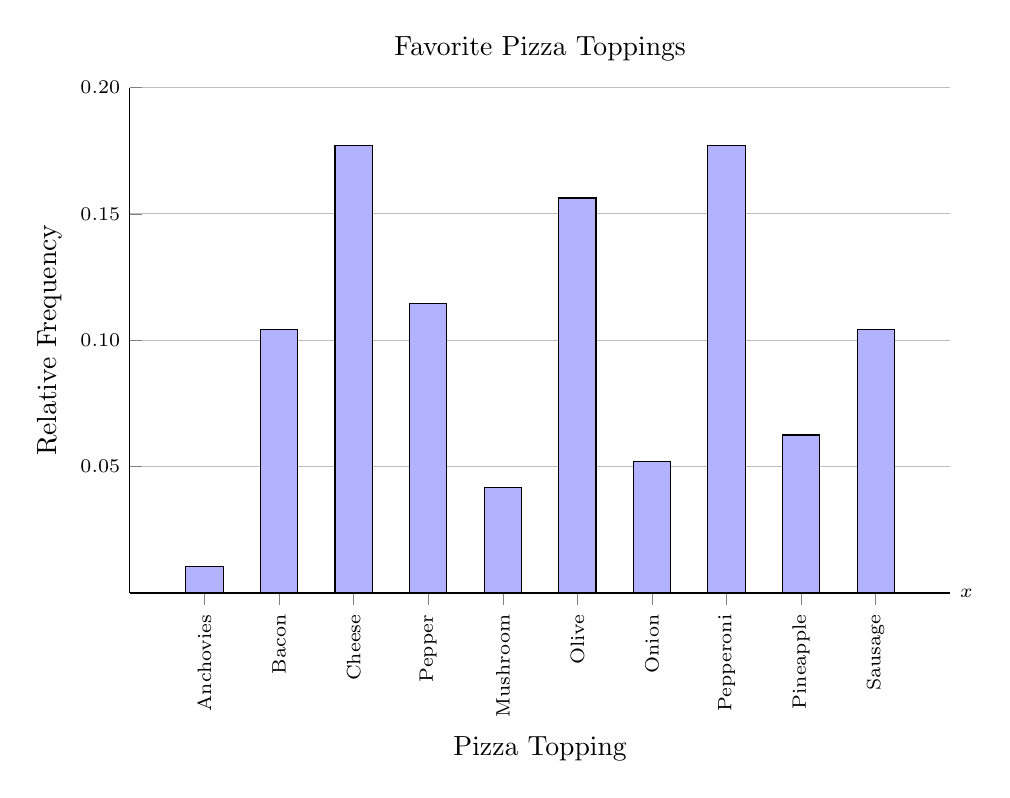
\begin{tikzpicture}[
    declare function={binom(\k,\n,\p)=\n!/(\k!*(\n-\k)!)*\p^\k*(1-\p)^(\n-\k);}
  ]
  \begin{axis}[
      axis lines*=left,
      no markers,
      xmin = 0, xmax=22, ymin=0, ymax=0.2,
      samples at={2,4,...,20},
      xtick={2,4,...,20},
      ytick={0.05,0.10,0.15,0.20}, 
      xticklabels={Anchovies,Bacon,Cheese,Pepper,Mushroom,Olive,Onion,Pepperoni,Pineapple,Sausage},
      ticklabel style={font=\scriptsize},
      xticklabel style={rotate=90},
      y tick label style={
        /pgf/number format/.cd,
        fixed,
        fixed zerofill,
        precision=2,
        /tikz/.cd
      },
      xlabel={Pizza Topping},
      ylabel={Relative Frequency},
      title={Favorite Pizza Toppings},
      enlargelimits=false,
      clip=false,
      grid = none,
      ymajorgrids=true,
      ybar=0pt, 
      bar width=1,
      width=12cm,
      height=8cm
    ]
    \addplot[fill=blue!30] coordinates { 
        (2,0.0104)
        (4,0.1042)
        (6,0.1771)
        (8,0.1146)
        (10,0.0417)
        (12,0.1563)
        (14,0.0521)
        (16,0.1771)
        (18,0.0625)
        (20,0.1042) 
    };
    \node[right] at (axis description cs: 1,0) {\scriptsize $x$};
  \end{axis}
\end{tikzpicture}
